%priprava posamezne ure
%tukaj zaporedoma napisemo{st. zaporedne ure}{datum}{naslov}{poglavje}{oblika dela}{pripomocki}
\begin{priprava}{}{}{Zaporedja}{Obrestni račun}{frontalna}{tabla}

% Jaz bi to ločila na svoje poglavje - Finančna matematika:)

Razlaga izrazov glavnica, obrestna mera ... Pač osnovno o bančništvu \dots

\naslov{Navadno obrestovanje}

Primer: na banko vložimo 500 € \didopomba{glavnica} po 3 \% letni obrestni meri. Koliko bomo imeli na računu čez 5 let?

$ G_0 = 500 $  € \\
$ p = 3 $ \% \didopomba{to pomeni, da nam po enem letu prištejejo 3 procente od glavnice} \\
Vsako leto nam tako prištejejo $ 0,03 \cdot 500 = 15 $ €. Zato imamo na računu po petih letih $ 500 + 5 \cdot 15 = 575 $ €.

Zdaj pa še v splošnem: \textcolor{rdeca}{$ G_n = G_0 + n \cdot \frac{p}{100} \cdot G_0 $}

\naslov{Obrestno obrestovanje}

Koliko pa dobimo, če obresti vsako leto pripišemo k novemu stanju? \didopomba{premislek pred izpeljavo -- dobimo manj ali več?}

$ G_0 \\
G_1 = G_0 + \frac{p}{100} \cdot G_0 = G_0 \cdot (1 + \frac{p}{100}) \\
G_2 = G_1 + \frac{p}{100} \cdot G_1 = G_1 \cdot (1 + \frac{p}{100}) = G_0 \cdot (1 + \frac{p}{100})^2 \\
G_3 = G_2 \cdot (1 + \frac{p}{100}) = G_0 \cdot (1 + \frac{p}{100})^3 \\
\cdots \\
\textcolor{rdeca}{G_n = G_0 \cdot (1 + \frac{p}{100})^n = G_0 \cdot r^n} $, kjer je $ r = 1 + \frac{p}{100} $ t.i. \textbf{obrestovalni faktor}.

Pri tej vrsti obrestovanja pa dobimo $ 500 \cdot 1,03^5 = 579,64 $ €. \didopomba{zaokrožujmo na 2 decimalni mesti. Še vedno pa ni veliko razlike, zato vzamemo primer z veliko glavnico ali pa večjim $ n $.}

Primerjava z novčičem, kako je eksponentna bolj naraščujoča: 2 centa obrestujemo 2000 let po 4 \% letni obrestni meri.
\begin{itemize}
    \item navadno obrestovanje: $ G_{2000} = 1,62 $ €
    \item obrestno obrestovanje: $ G_{2000} = 2,33 \cdot 10^{32} $ € (št. zvezd v vesolju???)
\end{itemize}

\vaje{
Vaje:
\begin{itemize}
    \item Za obe vrsti obrestovanj: Po kolikšni obrestni meri se obrestuje 250 €, da v 15 letih dobimo 362,07 €? Koliko let bi morali obrestovati, da bi presegli 400 €?
    \item Izračun le obresti in ne končnega stanja (to je razlika med začetnim in končnim stanjem) ipd.
\end{itemize}
}

\newpage

\naslov{Relativna in konformna obrestna mera}

Privzemimo obrestno obrestovanje.

Kaj pa se zgodi, če se obresti pripisujejo na pol leta ali vsak mesec? Ponavadi imamo podano letno obrestno mero $ p $, zato moramo za obdobje enega obrestovanja izračunati \textbf{relativno obrestno mero}: $ p $ delimo s številom obrestovanj na leto. Primeri:
\begin{itemize}
    \item letna obrestna mera: $ p $
    \item polletna obrestna mera: $ p/2 $
    \item mesečna obrestna mera: $ p/12 $
    \item dnevna obrestna mera: $ p/365 $
\end{itemize}

Če obresti pripišemo $ k $-krat na leto, skupaj pa $ m $-krat, je obrestovalni faktor tako enak
$$ r_k = 1 + \frac{p/k}{100}, $$
glavnica na koncu obrestovalnega obdobja pa
$$ G_m = G_0 \cdot r_k^m. $$

\vaje{
Vaje:
\begin{itemize}
    \item Obrestujemo glavnico 7000 € 5 let z mesečnim obrestovanjem ($ m = 5 \cdot 12 $). Koliko imamo na koncu? Kaj, če je obrestovanje dnevno ($ m = 5 \cdot 365$)?
    \item Koliko dobimo, če obrestujemo 20 000 € z letnim obrestovanjem in $ p $ = 4 \%, koliko pa, če obrestujemo mesečno? (20 800 € in 20 814,8 €) \didopomba{to je povod za obravnavo konformne obrestne mere}
\end{itemize}
}

Koliko bi pa morala biti prava mesečna obrestna mera, da bi bila po enem letu zneska enaka? Poglejmo splošen primer:

Z letnim obrestovanjem imamo po enem letu $ G \cdot r $. Sedaj pa nas zanima, kolikšna bi bila obrestna mera, če bi obrestovali $ k $-krat na leto, vendar bi na koncu želeli imeti enak znesek. Tej obrestni meri pravimo \textbf{konformna obrestna mera}.
$$ G \cdot r = G \cdot r_\text{konf}^k  \longrightarrow r_\text{konf} = 1 + \frac{p_\text{konf}/k}{100} = \sqrt[k]{r} \longrightarrow p_\text{konf} = 100 (\sqrt[k]{1+\frac{p}{100}} - 1)$$ \textcolor{red}{NAPAKA? Kam je izginil $ k $, a se zmnoži z njim ali ne???}

V našem primeru $ p_\text{konf} = 0,327 $ \% (relativna je $ \frac{4}{12} = 0,\overline{3}$).

\newpage

\naslov{Obročno odplačevanje (vplačila in izplačila)}

(Spet privezamemo obrestno obrestovanje.)

\textbf{Vplačevanje:} na banko $ n $ let vplačujemo konstantno vstoto $ a $. Prvič jo vplačamo danes (čas 0), zadnjič pa v čez $ n - 1 $ let \didopomba{slikca}. Koliko imamo takrat na računu? \didopomba{pomembno - kar smo že vplačali $a$-jev, se nam ustrezno obrestujejo sproti!}

\begin{figure}[h]
    \centering
    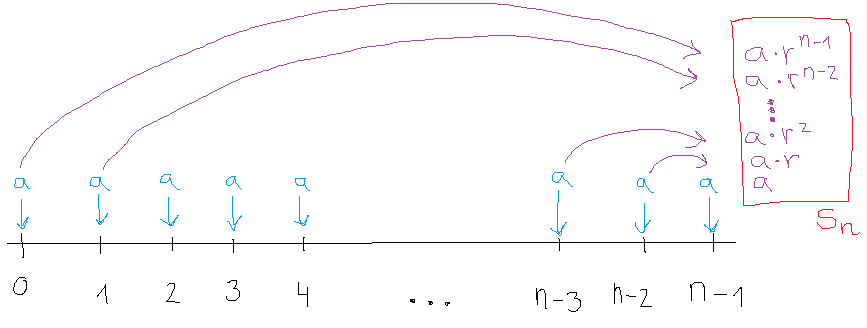
\includegraphics[width=\textwidth]{slike/vplačevanje.png}
\end{figure}

$$ S_n = ar^{n-1} + \ldots + a = \frac{a(r^n - 1)}{r - 1} $$

\textbf{Odplačevanje:} v času 0 smo si izposodili $ G $ denarja, ki ga odplačujemo $ n $ let po letnih obrokih, prvič po enem letu od posojila. Koliko mora znašati vsak obrok $ d $? \didopomba{Obrestovana glavnica mora biti enaka vsoti obrestovanih obrokov.}

\begin{figure}[h]
    \centering
    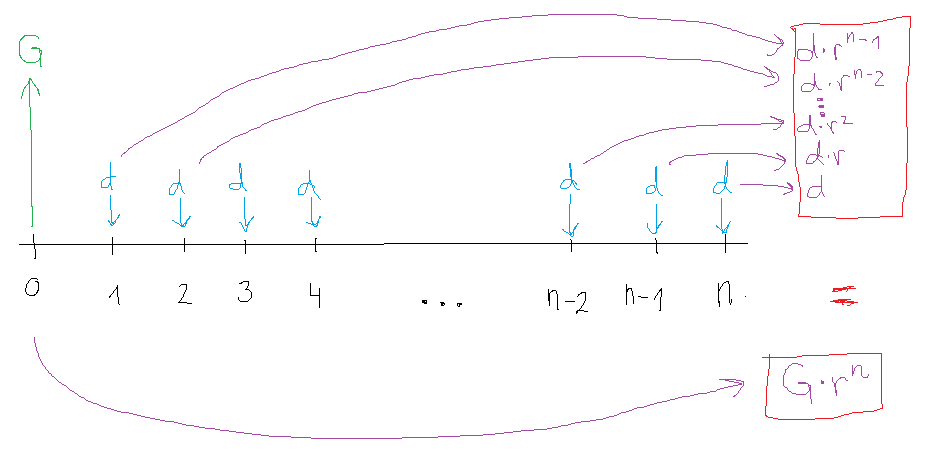
\includegraphics[width=\textwidth]{slike/odplačevanje.png}
\end{figure}

$$ G r^n =  dr^{n-1} + \ldots + d \rightarrow d = G\frac{r^n(r - 1)}{r^n - 1} $$

\didopomba{pomembno je, da se ne piflajo formul na pamet, ampak da jih razumejo. Da ne bo zmede, kolikokrat se obrestuje, pa kateri $ r $ in $ n $ vzeti, če nimamo le letnega obrestovanja in letnih izplačil, kateri čas vstavit itd.}

\end{priprava}